
\documentclass{article}
\usepackage{amsmath}
\usepackage[utf8]{inputenc}
\usepackage{subfig}
\usepackage{graphicx,tikz}
\usepackage{amsbsy}
\usepackage{hyperref}
%\title{Deep Reinforcement Learning for Perspective Taking Task}
\title{Perspective-Taking in Deep Reinforcement Learning Agents}

\author{
  Labash, Aqeel\\
  \texttt{aqeel.labash@gmail.com}\\
  \and
  Vicente, Raul\\
  \texttt{first2.last2@xxxxx.com}
  \and
  Aru, Jaan\\
  \texttt{first2.last2@xxxxx.com}
  \and
  Matiisen, Tambet\\
  \texttt{first2.last2@xxxxx.com}
  \and
  Tampuu, Ardi\\
  \texttt{first2.last2@xxxxx.com}
}
\date{March 2018} 
\usepackage{natbib}
\usepackage{graphicx}
\usepackage{makecell}
\usepackage{float}
\usepackage[%
    left=1.0in,%
    right=1.0in,%
    top=1.0in,%
    bottom=1.0in,%
    paperheight=11in,%
    paperwidth=8.5in%
]{geometry}%
\begin{document}
\maketitle
\section*{Abstract}
Perspective taking is the ability to take the point of view of another agent. This skill is not unique to humans but it is also displayed by other animals like chimpanzees. It is an essential ability to achieve efficient social interactions, including cooperation, communication, and competition. In this work, we present our progress toward building artificial agents with such abilities. To this end we created perspective-taking tasks, in which the environment is partially observable by agents who compete for a common resource. In this environment, we show that agents controlled by artificial networks learn via reinforcement learning to pass multiple tests that would benefit from perspective taking capabilities. We believe that building artificial agents with perspective taking faculties might help to reverse engineer how perspective taking task might be accomplished in our brains.


\section{Introduction}
Many decisions we take depend on others, what they think, what they believe, and what we know about what they know. This ability to understand and infer the mental states of others is called \textit{theory of mind} \cite{premack1978does} or mindreading \cite{apperly2011mindreaders}. Not only humans have the ability to take into consideration what others think and believe. In controlled experiments, it has been shown that chimpanzees can know what other conspecifics see and know \cite{hare2000chimpanzees}. Here we ask whether artificial intelligence (AI) agents controlled by neural networks \cite{Goodfellow-et-al-2016} could also learn to infer what other agents perceive and know. In particular, we test here the ability of an agent trained via reinforcement learning to acquire one essential part of \textit{theory of mind}: perspective taking. 

Perspective taking is looking at things from a perspective that differs from our own \cite{ryskin2015perspective}. It could be defined as "the cognitive capacity to consider the world from another individual's viewpoint" \cite{davis1983measuring}. According to Galinsky and colleagues, it is one of the social competencies that motivates social understanding in many contexts \cite{galinsky2008pays}.

\par When two persons are in a room that is familiar to both of them, they do not need to switch places to imagine what another can see and cannot see. However, this perspective taking ability is not unique to humans and has been observed in other animals like chimpanzees \cite{hare2000chimpanzees}. Chimpanzee social status is organized hierarchically (dominant, subordinate) \cite{goldberg1997genetic}. When there is food available that both can reach, the dominant monkey almost always gets it. In a series of experiments \cite{hare2000chimpanzees}  two chimpanzees were set into two separate cages facing the other with food positioned between them as shown in Figure \ref{tom.experiment} (left). The three conditions differed mainly in what the dominant and the subordinate monkeys can see. For example in the "subordinate door" condition one piece of food cannot be seen by the dominant chimpanzee. Can the subordinate take advantage of this fact? The results shown in Figure \ref{tom.experiment} (right) demonstrate that the subordinate animal indeed obtained more food in this condition. Hence, the it was able to take into account what the dominant chimpanzee could and couldn't see, i.e. take the perspective of the dominant chimpanzee. For other experiments and details see for example \cite{hare2000chimpanzees, de2016we, tomasello2009cultural}.  

\begin{figure}[!ht]
\begin{center}
\includegraphics[scale=0.3]{figures/tom_experiment_1.png}
\includegraphics[scale=0.3]{figures/tom_experiment_1_results.png}
\caption{Left: three different positions for the food with different obervability (food indicated by black ellipses, cage walls indicated by lines). Right top: Average percentage of food eaten by subordinate for different food positions. Right bottom: the average percentage based on food visibility condition. Figure from \cite{hare2000chimpanzees}.}
\label{tom.experiment}
\end{center}
\end{figure}

In this work, we designed a reinforcement learning environment \texttt{APES} that allowed us to simulate the experiments described in \cite{hare2000chimpanzees} where a subordinate chimpanzee chose whether to go for food or not depending on the observability of the food by the dominant chimpanzee. The aim of the present work is to study whether an AI agent controlled by a neural network can learn to solve similar perspective taking task using reinforcement learning (RL).

RL is a branch of AI that allows an agent to learn by trial and error while interacting with the environment. In particular, the agent must learn to select the best action in each specific state to maximize its cumulative future reward \cite{sutton1998reinforcement}. The agent could be an autonomous robot \cite{lin1993reinforcement,yang2004multiagent,riedmiller2009reinforcement} or a character in video game \cite{mnih2015human} or even computer simulations based of biological systems \cite{amigoni2007multiagent}. 

\par 
The idea behind learning by interacting with an environment is inspired from how human and animal infants learn from the rich cause-effect or action-consequence structure of the world \cite{sutton1998reinforcement,thorndike1911animal,schultz1997neural}. Therefore, RL is a biologically plausible mechanism for learning certain associations and behaviors. 

By this work we do not claim that RL captures all aspects of perspective taking or is the exact model of how perspective taking is learned in biological organisms (Aru \& Vicente, submitted). However, we hope that understanding the capabilities and limitations of RL in acquiring perspective taking skills will lead to a better algorithmic understanding of perspective taking also in biological organisms.

\subsection{Related work}
Recently, Rabinowitz and colleagues have proposed a neural network to model agents behavior in a grid world. The proposed network is trained using metalearning; in a first stage the network is trained to learn some priors for the behavior of different types of agents to subsequently speed up the learning of modeling a specific agent from a smaller number of behavioral observations. Their approach was a first step to induce theory of mind faculties in AI agents that were indeed able to pass some relevant tests for theory of mind skills. However, as the authors themselves note in their paper, their current approach is limited in several important aspects that require future work. To name a few, the observer agent learning to model the behavior of others is trained in a supervised manner, it has full observability of the environment and the other agents, and it is not itself a behaving agent. 

In this paper we are interested in the emergence of perspective-taking faculties in behaving agents trained via reinforcement learning with partial observability. We believe that these are more plausible conditions to model how humans and other animals might develop some perspective taking abilities. 


\section{Methods}
To train a model capable of solving tasks that require perspective taking, three ingredients were utilized. First, an environment to simulate the task. Second, a neural network model. Third, a training strategy for acquiring perspective taking capacity. It is not a straightforward task that can easily be learned end to end.

\subsection{Environment}
%\textbf{General speaking about the envrionment functionality like you can use 10 agents etc .. }
To create our experiments we used Artificial Primate Environment Simulator (\textit{APES}) \cite{APES}. This environment allows to simulate a grid world and populate it with multiple agents and different items using a binary environment representation. \textit{APES} also includes vision algorithms for the agents that allow building vision barriers (obstacles) and calculate vision based on agents' location, orientation and vision range and angle. For more details the reader can access the \href{https://github.com/aqeel13932/APES}{GitHub repository}

For the perspective learning task,we created an $11\times11$ grid world environment. The elements in the world have certain places to spawn in, in every episode with Dirichlet distribution. Figure (\ref{fig:probabilities}) shows the elements' possible locations at the beginning of every episode. In all experiments that have a dominant agent \(A_{dom}\) it always moves in random steps towards unexplored area. Once \(A_{dom}\) spots the food (reward) it moves towards it immediately using deterministic path-planning.
\begin{figure}[H]
    \centering
    \includegraphics[scale=0.5,trim={0cm 1cm 0cm 0cm},clip]{figures/probabilities.png}
    \caption{The possible start positions for each element in the environment. Agent 1 is the subordinate, Agent 2 is the dominant.(Best seen in colors.)}
    \label{fig:probabilities}
\end{figure}

\subsection{Model}\label{model}
We kept the model simple and straightforward. We used a feedforward neural network, see Figure \ref{fig.model}. Our model estimates state value and advantages, which is similar to dueling network \cite{DBLP:journals/corr/WangFL15}, but instead of splitting the last layer we used all of it for value and advantages. Each experiment generated two models: 1) training model, which is updated every time step, 2) target model which $\tau$-averaged copy of training model weights every step (\(\theta^{-} = \theta \tau + \theta^{-} (1-\tau)\)).
  \begin{equation} \label{eq:model.mod}
    Q(s,a;\theta,\alpha,\beta) = V(s;\theta,\beta) +\left( A(s,a;\theta,\alpha) - \underset{a' \in A}{\max}A(s,a';\theta,\alpha) \right)
  \end{equation}
\begin{figure}[!ht]
\begin{center}
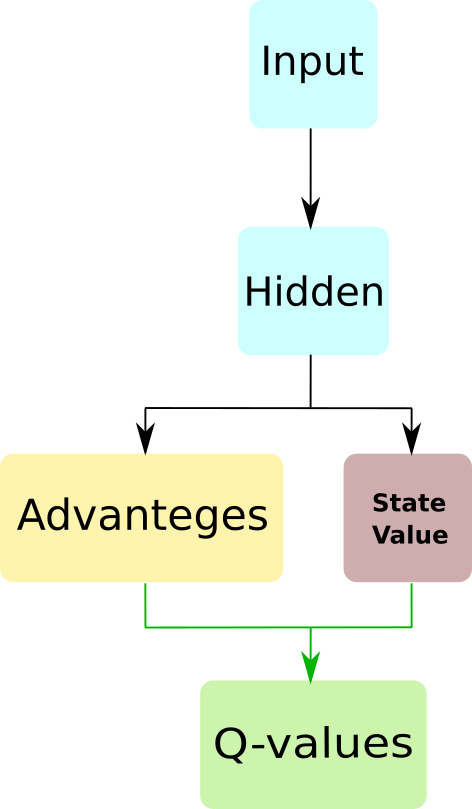
\includegraphics[scale=0.5]{figures/model1.png}
\caption{Feedforward network where the connections between the last layer and the Q-values is regulated by formula \ref{eq:model.mod}}
\label{fig.model}
\end{center}
\end{figure}

 \par We fed \label{network.input} agent visual field as input to the agent's network in the form of binary feature vectors. Separate binary maps were used for agent's position, dominant agent's position, food position, observed area and obstacles' position. In addition a one-hot vector of size 4 per agent was added representing the agent's direction of vision.

\par We used replay memory which is a common practice when deep learning is used for RL tasks\cite{mnih2015human}.

\subsection{Perspective-taking Task}
The task we used included two agents: dominant $A_{dom}$ and subordinate $A_{sub}$. $A_{dom}$ and $A_{sub}$ are placed in an arena that contains obstacles $O$ that block vision and food $F$, which is the reward. $A_{sub}$ needs to reach the food while keeping a certain minimal distance from the $A_{dom}$, otherwise it will get punished. $A_{dom}$ is driven by a deterministic algorithm to find the food. 
We trained $A_{sub}$ in a curriculum learning scheme.
Curriculum learning consists of training an agent on a sequence of tasks of increasing complexity to improve the speed of learning in a more complex task \cite{narvekar2016curriculum}. We defined two tasks explained in the following sections where we trained the agent first to find the food (Task 1) after that to avoid the dominant (Task 2).
\subsubsection{Task 1: finding the food} \label{task1}
In this first stage of learning the only task \(A_{sub}\) had to perform was to find the food. This task might look easy but when we consider the limited vision and the obstacles it gets more complicated. Without a memory the agent has to act depending on the immediate vision of field. This task optimize \(A_{sub}\) to look for the food and approach it. To make the task reasonably challenging, the obstacle will spawn randomly within a specific region as shown in Figure \ref{fig:probabilities}. In this task there is no $A_{dom}$ and input map representing the dominant agent's location is set to all zeros at all times. The agent receives a -0.1 reward per time step regardless of the chosen action and 1000 for consuming food.
\subsubsection{Task 2: avoiding dominant agent}\label{task2}
Here, we trained the subordinate agent to behave in the presence of a dominant agent. The dominant punishes the suboordinate with -100 reward points whenever it comes closer than 2 steps from the dominant and is within its field of vision (i.e. if the dominant sees it). 
 
\subsection{Behavioral test cases}\label{agents.behavior}
We created 10 behavioral tests cases that cannot be accomplished without perspective taking abilities. In those test cases we tried to cover all the possible factors. Mainly we stabilized the positions of all elements (dominant, subordinate, food, obstacle) with the exception of one of them at a time.
In addition to different types we tried 4 variations of each test case to make sure that results were not just a statistically calculated. 

We created 10 behavioural test cases that cannot be solved without perspective-taking abilities. The test cases are illustrated on Figure XXX. In each case, we set the agents and obstacles to specific places and orientations to create specific situations. For these situations we know what is the expected (optimal) behaviour of $A_{sub}$. We compare the actual behaviour with this expected behaviour. To further confirm if the agent indeed successfully solves these situations, 4 variations of each case were run. The variations differ in spatial setup, but same behaviour is expected. The results hold for all variations run.
\begin{itemize}

\item \textbf {Test case 1:} in this test scenario, illustrated on Figure \ref{fig.tc.1}a, the subordinate agent \(A_{sub}\) is supposed to go for the food since the food is unobserved by the dominant agent \(A_{dom}\). At the same time \(A_{sub}\) and \(A_{dom}\) cannot see each other. Environment in Figure \ref{fig.tc.1}.

\item \textbf {Test case 2:} \(A_{sub}\) can see the food and can see\(A_{dom}\). The favored behavior from \(A_{sub}\) is to avoid the food since \(A_{dom}\) can see the food. Environment in Figure \ref{fig.tc.2}.

\item \textbf {Test case 3:} \(A_{sub}\) is supposed to go for the food in case \(A_{dom}\) was not spotted in its field of vision before eating the food. Environment in Figure \ref{fig.tc.3}.

\item \textbf {Test case 4:} \(A_{sub}\) and \(A_{dom}\) can see each other while only \(A_{sub}\) can see the food. Hence, \(A_{sub}\) is supposed to go for the food. Environment in Figure \ref{fig.tc.4}.

\item \textbf {Test case 5:} similar to test case 2 where \(A_{sub}\) with exception that \(A_{dom}\) is more distanced from the food. Environment in Figure \ref{fig.tc.5}.

\item \textbf {Test case 6:} agents can see each other but only \(A_{sub}\) can see the food. Similar case to Figure \ref{fig.tc.4} but \(A_{dom}\) here is closer to the food. The expected behavior is to go for the food. Environment in Figure \ref{fig.tc.6}.

\item \textbf {Test case 7:} both agents can see the food but not each other. \(A_{sub}\) should go to food as long as \(A_{dom}\) is not spotted before taking the last action. Environment in Figure \ref{fig.tc.7}

\item \textbf {Test case 8:} \(A_{sub}\) can see both food and \(A_{dom}\) while the latter can see neither \(A_{sub}\) nor the food. \(A_{sub}\) supposed to go for the food as the dominant is looking away. Environment in Figure \ref{fig.tc.8}.

\item \textbf {Test case 9:} \(A_{sub}\) see all other elements while \(A_{dom}\) does not.\(A_{sub}\) is supposed to go for the food. Environment in Figure \ref{fig.tc.9}

\item \textbf {Test  case 10:} \(A_{sub}\) and \(A_{dom}\) can see the food, but can not see each other. \(A_{sub}\) is expected to go for the food as long as it has not spotted the dominant Figure \ref{fig.tc.10}.
\end{itemize}




\subsection{Training}
We trained our models using curriculum learning. First we trained the models on task 1 for 2 million steps. Exploration rate started at 1 and decreased to reach 0.1 after 1,5 million steps. In a second phase of learning, we trained the model on task 2 for 500 000 steps with exploration rate fixed at 0.1. We explored many values for hyper-parameters shown in Table \ref{tab:best.hyp}. Typically we ran grid search procedure for different combinations of pairs of parameters.
\par Choosing the best hyper-parameters was based on the training average reward over multiple random seeds. Table \ref{tab:best.hyp}  shows the best hyper-parameters that fit our task. For the neural network implementation we used the \texttt{Keras} library \cite{chollet2015keras}.

\begin{table}[H]
    \centering
    \begin{tabular}{*{2}{|c|}}
    \hline
         \textbf{Replay memory size}& 100K\\
         \hline
         \textbf {\# layers }&1\\
         \hline
         \textbf {Hidden nodes}&100\\
         \hline
         \(\boldsymbol{\tau}\)&0.001\\
         \hline
         \textbf {Advantage}&\texttt{max} \\
         \hline
         \textbf {Activation}&\texttt{tanh}\\
         \hline
         \(\boldsymbol{\epsilon}\)&0.01\\
         \hline
         \textbf {Batch size}&32\\
         \hline
         \textbf {Training repeat} &1\\
    \hline
    \end{tabular}
    \caption{best hyper-parameters}
    \label{tab:best.hyp}
\end{table}

Those hyper-parameters performed the best over multiple random seeds. We used them for the rest of the experiments.

\section{Results}

\subsection{Behavioral test cases}
Our goal is to study whether deep RL agents could learn to infer what other agents can and cannot perceive. We tested our agents with 10 test cases designed to be accomplishable only with perspective taking abilities. In those test cases we paused the dominant agent's movement completely to see the emerged behavior from the subordinate. The following figures illustrate the test cases and the agent's behavior. The legend of each figure explains the situation and the behavior in more detail.

\def \xx{0.15}
%\begin{changemargin}{-1cm}{-1cm}
\newgeometry{left=1cm,right=1cm,bottom=2cm,top=1cm}
\begin{figure}[H]
\begin{center}
\begin{table}[H]
    \centering
    \begin{tabular}{|p{9cm}|p{9cm}|}
    \hline
        \subfloat[]{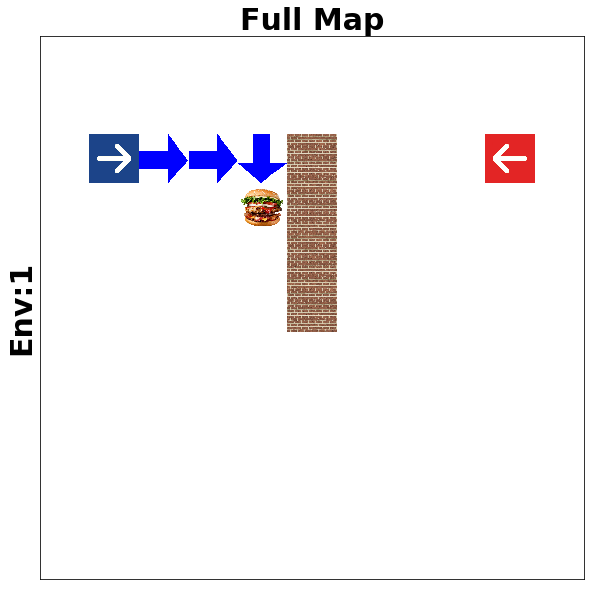
\includegraphics[scale=\xx]{figures/ENV:1_FM.png}}
        \subfloat[]{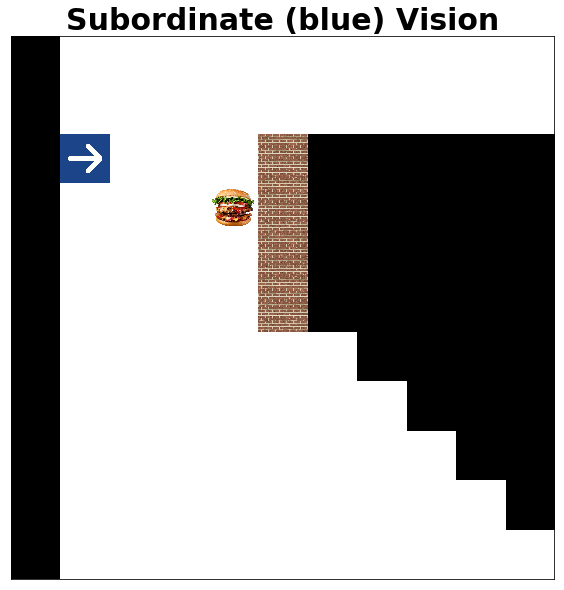
\includegraphics[scale=\xx]{figures/ENV:1_AI.png}}
        \subfloat[]{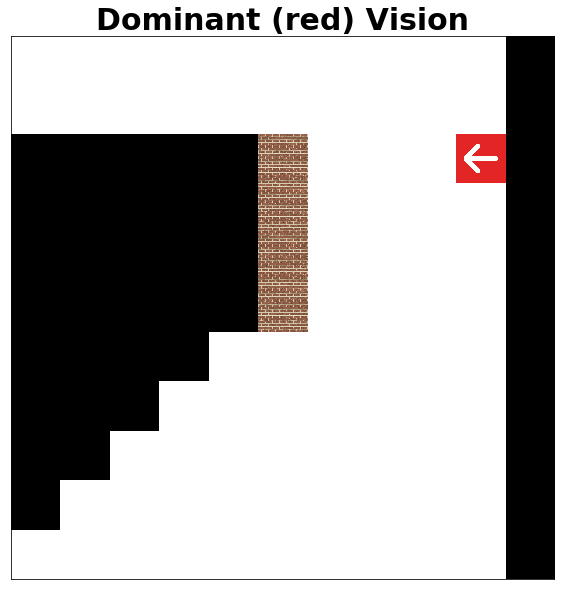
\includegraphics[scale=\xx]{figures/ENV:1_DM.png}}&
        \subfloat[]{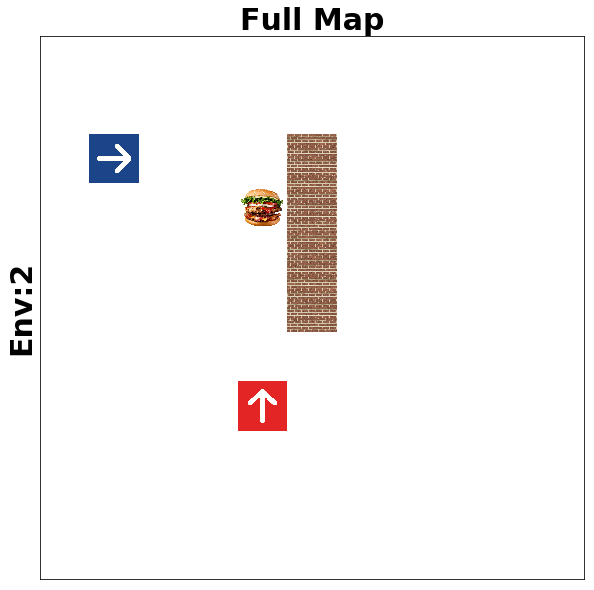
\includegraphics[scale=\xx]{figures/ENV:2_FM.png}}
        \subfloat[]{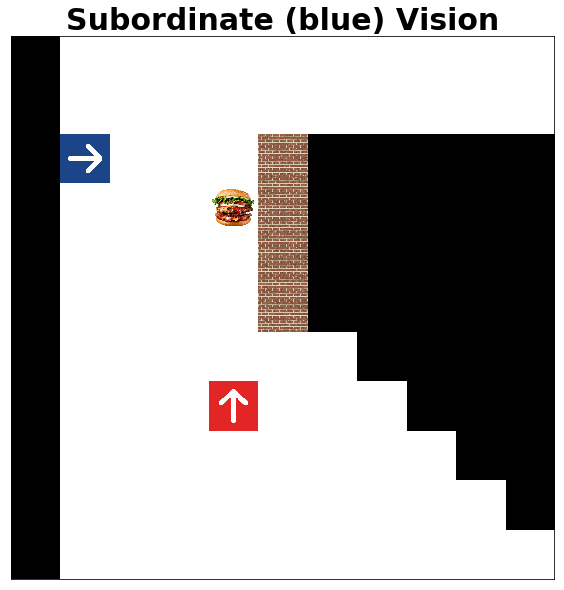
\includegraphics[scale=\xx]{figures/ENV:2_AI.png}}
        \subfloat[]{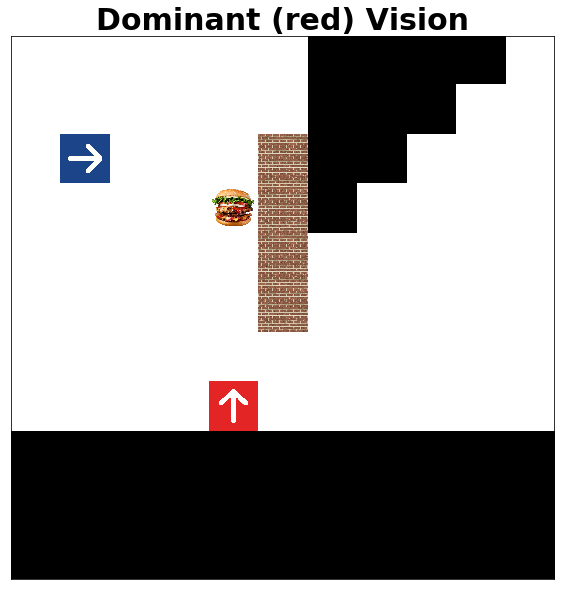
\includegraphics[scale=\xx]{figures/ENV:2_DM.png}}  \\
        \hline
         \textbf {Test  case 1(a,b,c):} \(A_{sub}\) did not see the dominant as the dominant was behind the obstacle. \(A_{sub}\) went for the food in 4 steps. The trajectory was optimal.  For this test case \(A_{sub}\) achieved the expected behavior.&
         \textbf{Test  case 2(d,e,f):} \(A_{sub}\) avoided the food although the food is in the same position as in \texttt{Test case 1}. The only difference is the dominant position and direction: the dominant can see the food. The observed behavior is also what one would expect from an agent with the perspective taking ability.
        \\
        \hline
        \subfloat[]{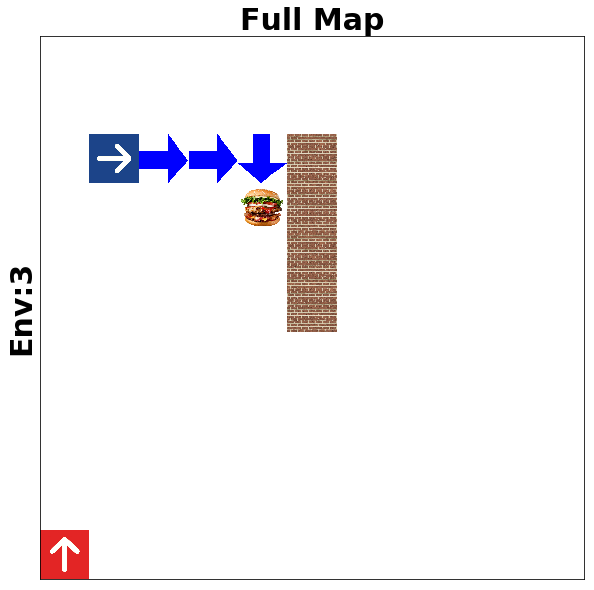
\includegraphics[scale=\xx]{figures/ENV:3_FM.png}}
        \subfloat[]{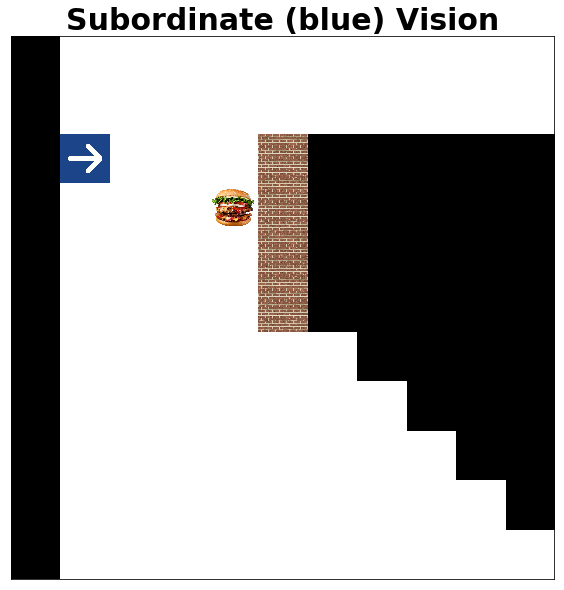
\includegraphics[scale=\xx]{figures/ENV:3_AI.png}}
        \subfloat[]{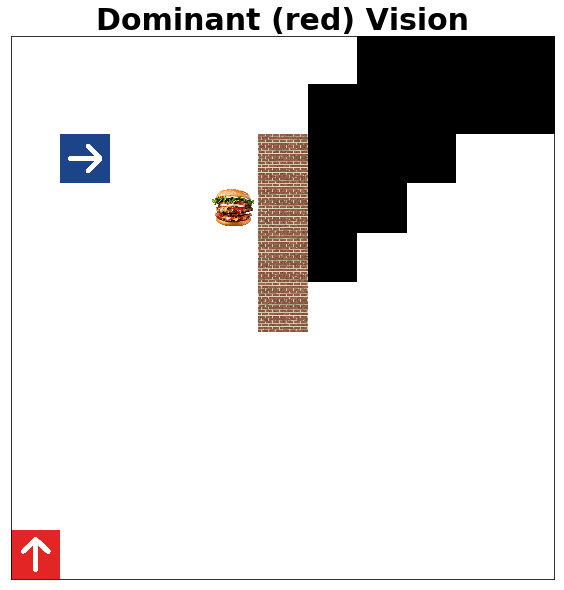
\includegraphics[scale=\xx]{figures/ENV:3_DM.png}}&
        \subfloat[]{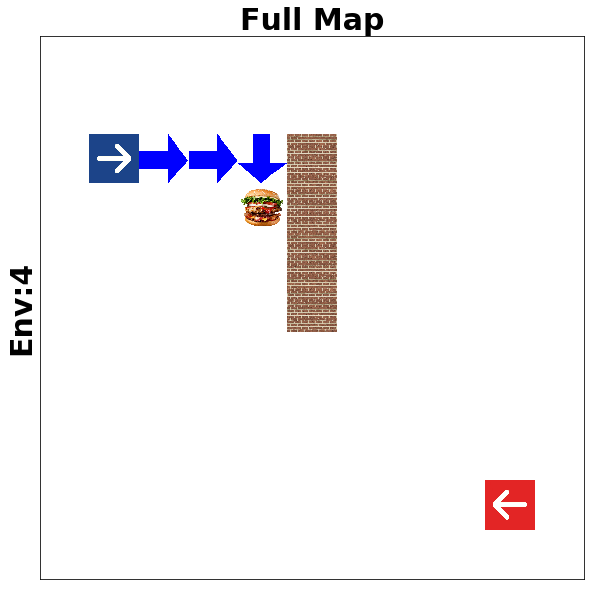
\includegraphics[scale=\xx]{figures/ENV:4_FM.png}}
        \subfloat[]{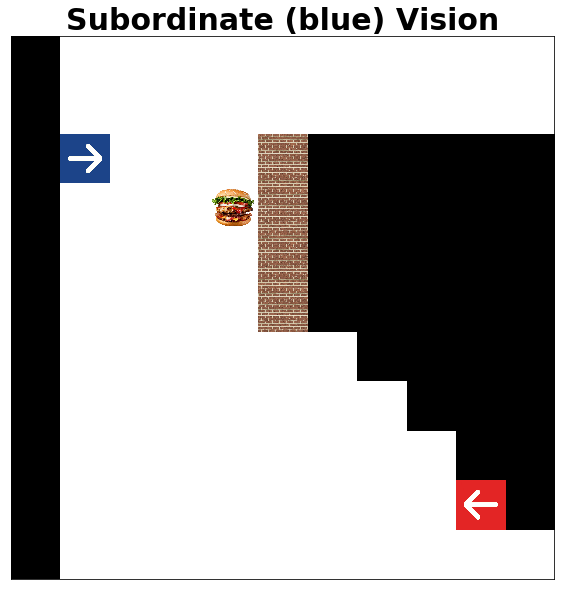
\includegraphics[scale=\xx]{figures/ENV:4_AI.png}}
        \subfloat[]{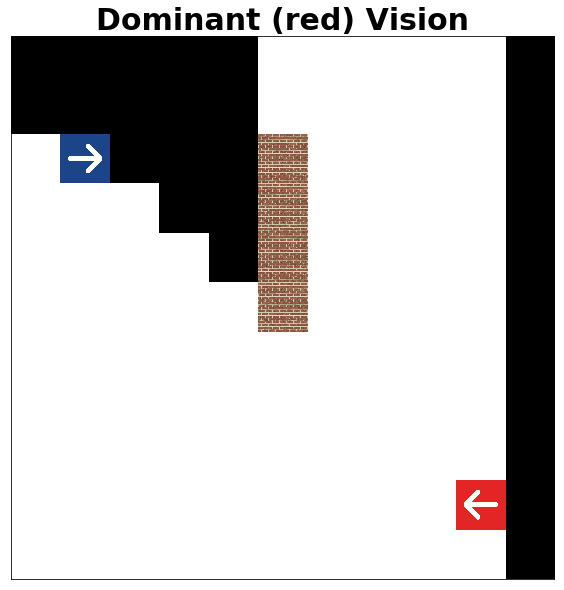
\includegraphics[scale=\xx]{figures/ENV:4_DM.png}}\\
        \hline
         \textbf{Test  case 3(g,h,i):} \(A_{sub}\) went for the food, although the dominant is there and able to see everything. Notice however that $A_{dom}$ was unspotted by $A_{sum}$ until the very last step of eating the food.  This behavior is expected to also happen with perspective taking capable agents.
        &
          \textbf{Test  case 4(j,k,l)}: in this case the subordinate reached for the food. Although the dominant was looking toward the subordinate, the food was not visible for the dominant. This behavior matches what an agent with perspective taking would do.
        \\
        \hline
        \subfloat[]{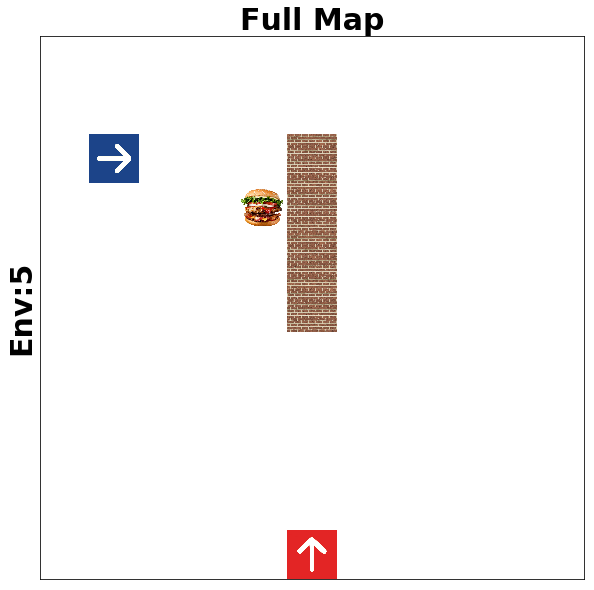
\includegraphics[scale=\xx]{figures/ENV:5_FM.png}}
        \subfloat[]{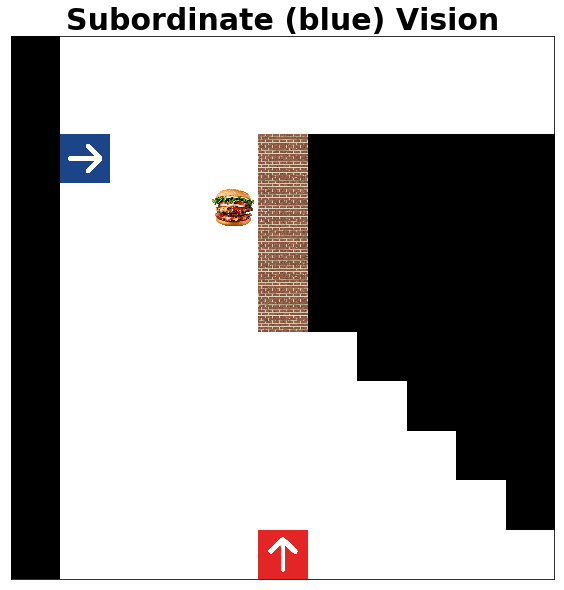
\includegraphics[scale=\xx]{figures/ENV:5_AI.png}}
        \subfloat[]{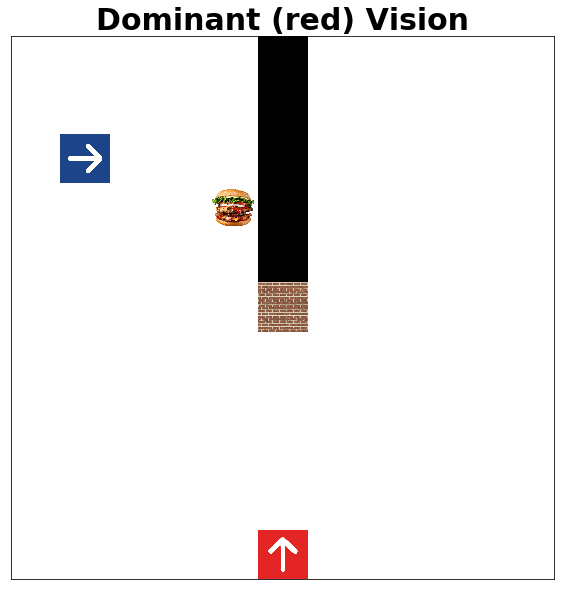
\includegraphics[scale=\xx]{figures/ENV:5_DM.png}}&
        \subfloat[]{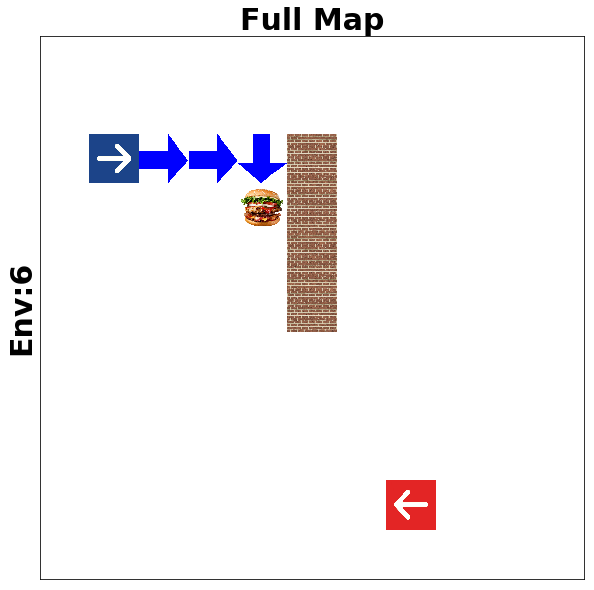
\includegraphics[scale=\xx]{figures/ENV:6_FM.png}}
        \subfloat[]{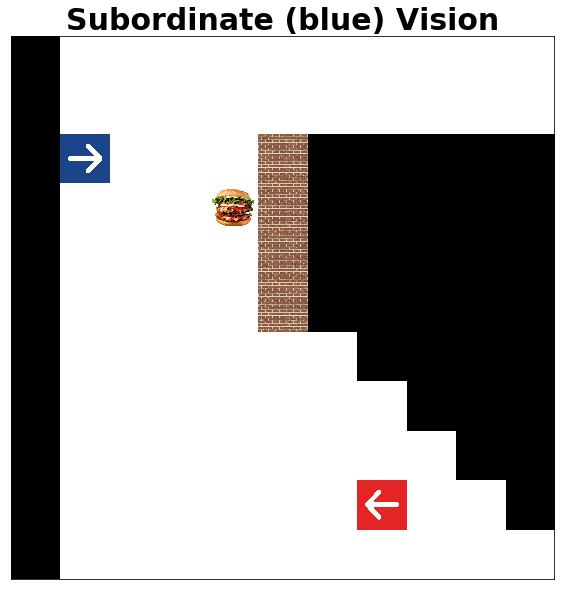
\includegraphics[scale=\xx]{figures/ENV:6_AI.png}}
        \subfloat[]{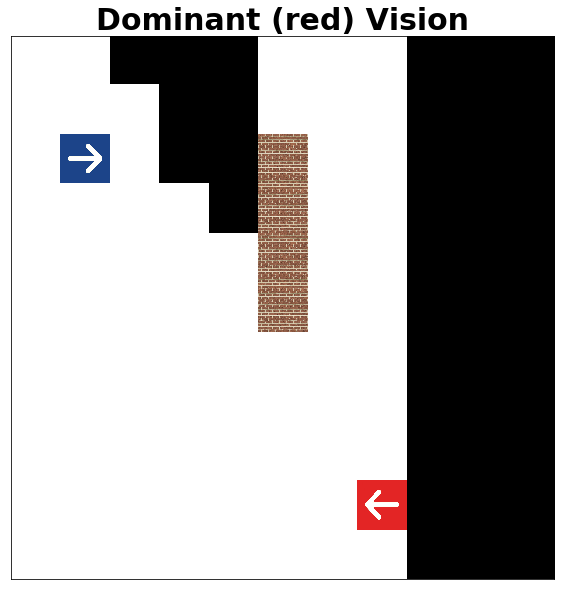
\includegraphics[scale=\xx]{figures/ENV:6_DM.png}}\\
        \hline
         \textbf{Test case 5(m,n,o):} just like test case 2 but \(A_{dom}\) is farther away from food. 
        &
        \textbf{Test  case 6(p,q,r):} this test case is identical to test case 4 with the change in the distance between the dominant and the food. Although the dominant is closer to the food, food is still hidden from its visual field. The subordinate went for the food in this experiment which is a behavior to expect from an agent capable of perspective taking ability.
        \\
        \hline
    \end{tabular}
    \caption{a) Full map of the world where the square blue arrow on the left represent the subordinate \(A_{sub}\) and the square red arrow on right represent the dominant \(A_{dom}\).  The filled blue continous arrows show agent trajectory to reach the food. b) Show \(A_{sub}\) vision. The input to the subordinate network was only information extracted from (b) as explained in section (\ref{model}) where the black area represent unobservable area. c) Show the observed and unobserved area by the dominant (although the dominant does not use a neural network). No information from (a) or (c) were fed to \(A_{sub}\) network.}
    \label{tab:my_label}
\end{table}
    \caption{Figure caption}
    \label{fig.tc.1}
    \label{fig.tc.2}
    \label{fig.tc.3}
    \label{fig.tc.4}
    \label{fig.tc.5}
    \label{fig.tc.6}
\end{center}
\end{figure}

\begin{figure}[H]
\begin{center}
\subfloat[]{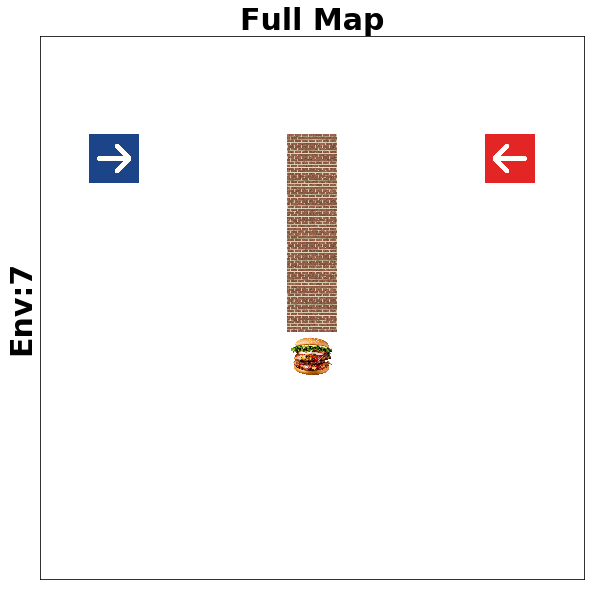
\includegraphics[scale=\xx]{figures/ENV:7_FM.png}}
\subfloat[]{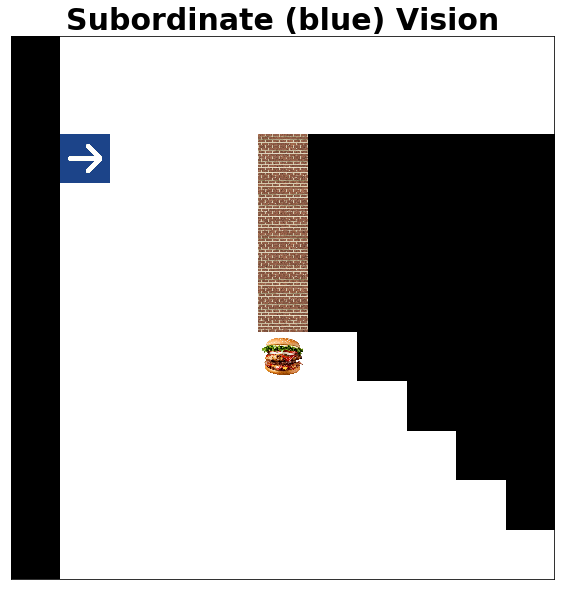
\includegraphics[scale=\xx]{figures/ENV:7_AI.png}}
\subfloat[]{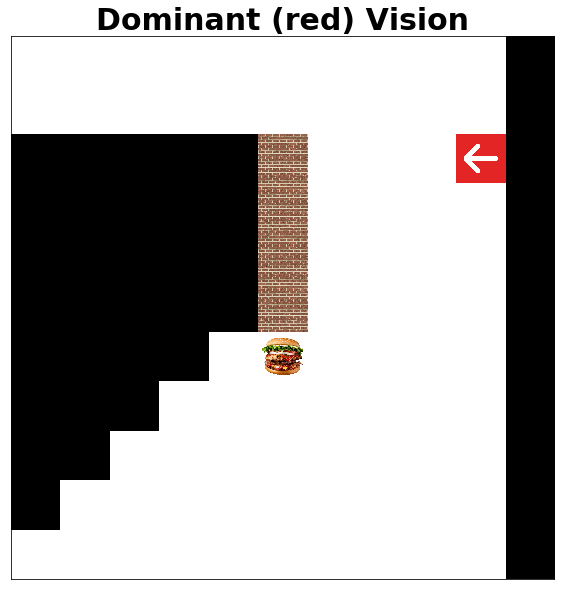
\includegraphics[scale=\xx]{figures/ENV:7_DM.png}}
\subfloat[]{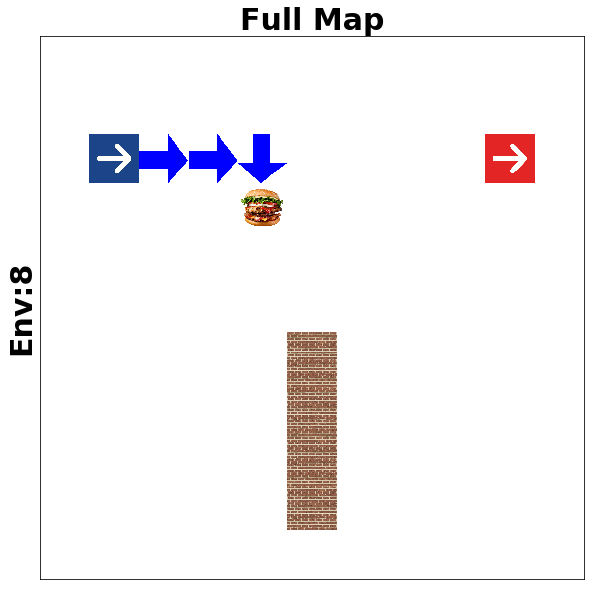
\includegraphics[scale=\xx]{figures/ENV:8_FM.png}}
\subfloat[]{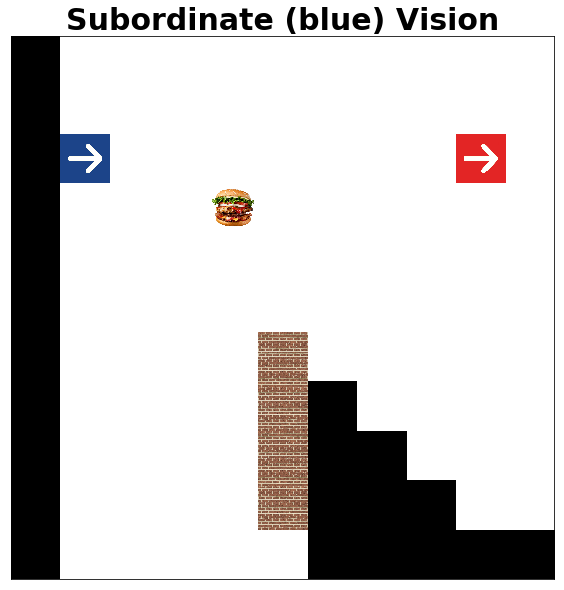
\includegraphics[scale=\xx]{figures/ENV:8_AI.png}}
\subfloat[]{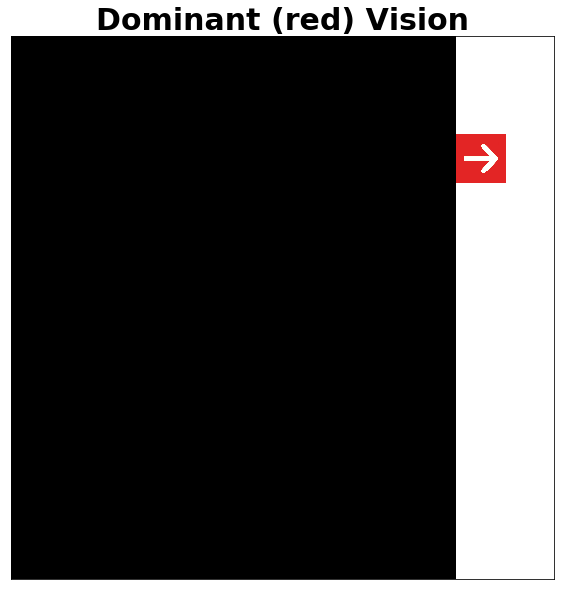
\includegraphics[scale=\xx]{figures/ENV:8_DM.png}}\\
\subfloat[]{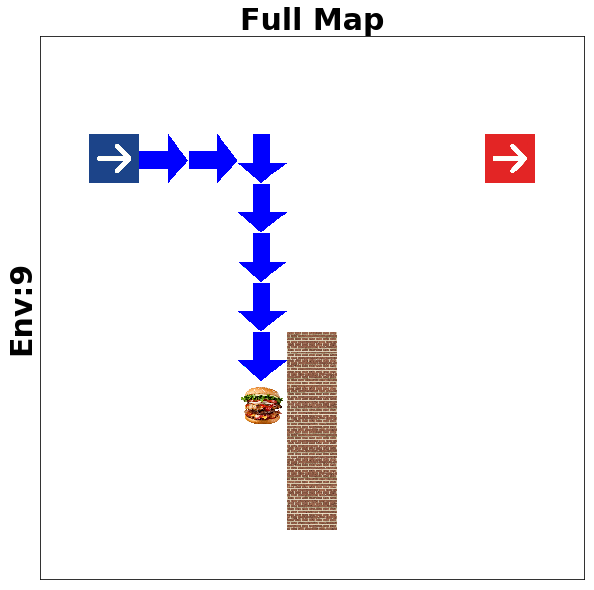
\includegraphics[scale=\xx]{figures/ENV:9_FM.png}}
\subfloat[]{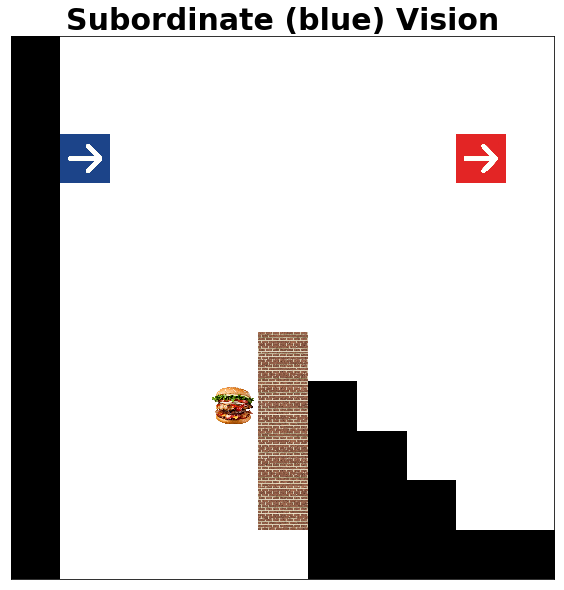
\includegraphics[scale=\xx]{figures/ENV:9_AI.png}}
\subfloat[]{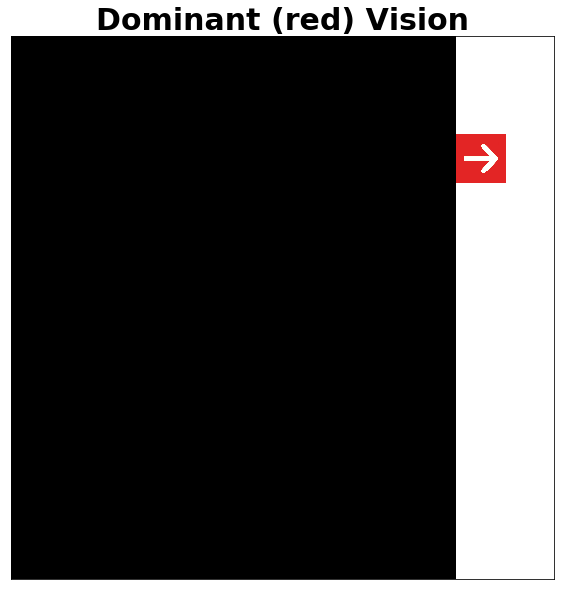
\includegraphics[scale=\xx]{figures/ENV:9_DM.png}}
\subfloat[]{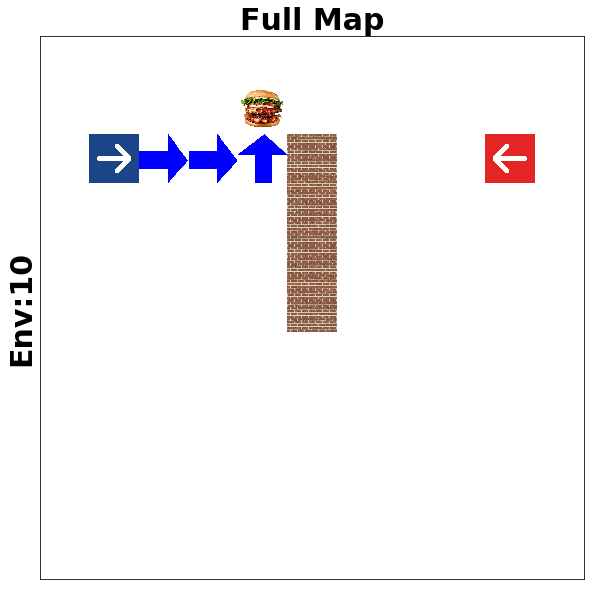
\includegraphics[scale=\xx]{figures/ENV:10_FM.png}}
\subfloat[]{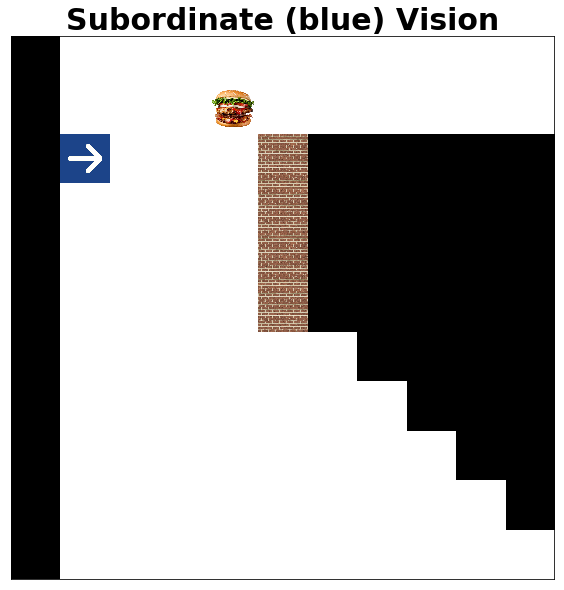
\includegraphics[scale=\xx]{figures/ENV:10_AI.png}}
\subfloat[]{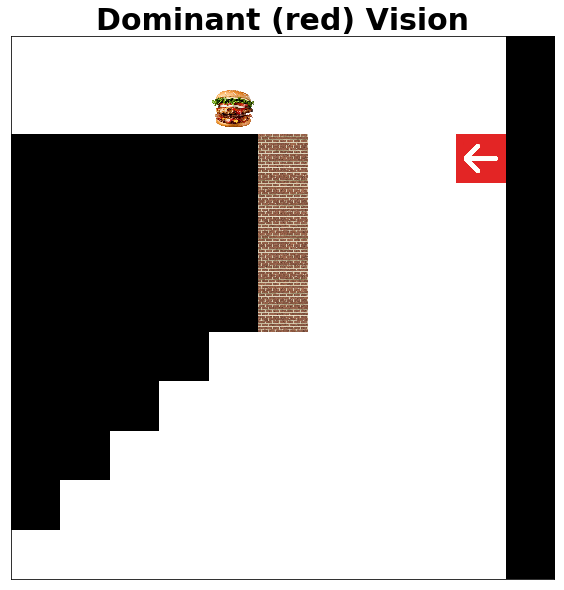
\includegraphics[scale=\xx]{figures/ENV:10_DM.png}}
\caption{\textbf {Test  case 7(a,b,c):} \(A_{sub}\) avoided the food although the dominant was not spotted in its field of view. It might be the case that food position is dangerous from previous experience while training. \textbf{Test  case 8(d,e,f):} subordinate went for the food in this test case. Since the dominant was looking in the other direction, the food was not spotted by the dominant. Hence it is plausible to go for the food. \textbf{Test  case 9(g,h,i):} in this case we changed the food location and the obstacle where they are not seen by dominant. The subordinate retrieved the food successfully which is a behavior coinciding with perspective knowledge. \textbf{Test  case 10(j,k,l):} In this test case \(A_{sub}\) should or should not go to the food based on the trajectory followed. As we can see \(A_{dom}\) was never spottes by \(A_{sub}\) and therefore the behaviour is as expected by and agent with perspective taking ability.}
\label{fig.tc.7}
\label{fig.tc.8}
\label{fig.tc.9}
\label{fig.tc.10}
\end{center}
\end{figure}

\restoregeometry

Our subordinate agent solved all of these test cases successfully, demonstrating a capability for perspective taking. To control for the robustness of the results we included 4 sets of variations to the test cases where we shifted one or many elements by a pixel: 1) Shift all elements, 2) Shift dominant, 3) Shift Subordinate only, 4) Shift food position. In 95\% of these variations we observed similar results to the main results, hence confirming that our agent is not fooled by small variations of the data.

In table \ref{table:Tests} we summarize the results and show the expected behavior compared to the model behavior.
\begin{table}[H]
    \centering
    \begin{tabular}{|{c}||*{10}{c|}}
    \hline
    Test case&1&2&3&4&5&6&7&8&9&10\\
    \hline
    Video link&1&2&3&4&5&6&7&8&9&10\\
    \hline
    Figure&\ref{fig.tc.1}&\ref{fig.tc.2}&\ref{fig.tc.3}&\ref{fig.tc.4}&\ref{fig.tc.5}&
    \ref{fig.tc.6}&\ref{fig.tc.7}&\ref{fig.tc.8}&\ref{fig.tc.9}&\ref{fig.tc.10}\\
    \hline    
     \makecell{Dominant position \\ Food and obstacle \\ position}&DP&DP&DP&DP&DP&DP&FO&FO&FO&FO\\
    \hline
    \makecell{Expected behavior:\\Go or No}&Go&No&Go&Go&No&Go&No&Go&Go&Go\\
    \hline
    Actual behavior&Go&No&Go&Go&No&Go&No&Go&Go&Go\\
    \hline
    \end{tabular}
    \caption{show the test cases types (stabilizing everything but changing dominant position DP, or changing food and obstacle FO) and the expected behavior from the subordinate in each one. Last row show the actual behavior performed by the model.}
    \label{table:Tests}
\end{table}

\subsection{Inside the network}
The first step toward looking inside the network was checking T-SNE over the weights and activations. Doing that will reveal the clusters and give us the opportunity to find out the pattern they are grouped by if possible. In Figure (\ref{fig.TSNE_Weights}) we plot T-SNE over all the hidden nodes weights where we considered each hidden node a vector of length 633 (input size). We can notice clearly two clusters which make us believe a simpler network might also be sufficient to do the job (similar neuron might be replaced by averaged one) (Although we tried with less size but never succeeded).
\begin{figure}[H]
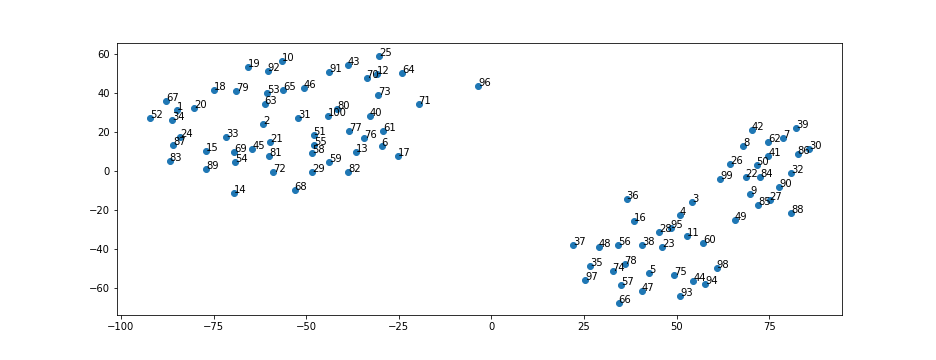
\includegraphics[scale=0.5,trim={3.5cm 0cm 2cm 0.5cm},clip]{figures/TSNE_Weights.png}
\caption{T-SNE over nodes in hidden layer, where we consider the weights from input are the node features.}
\label{fig.TSNE_Weights}
\end{figure}

We chose the neurons with the strongest positive and negative weights to state value and tried to see what those neurons represent. To visualize this we drew the weights between the inputs and those two neurons. Figures (\ref{fig.PN_61},\ref{fig.SN_61}) show the neuron with highest positive weight and Figure (\ref{fig.PN_76},\ref{fig.SN_76}) show the neuron with highest negative weight.  


\begin{figure}[H]
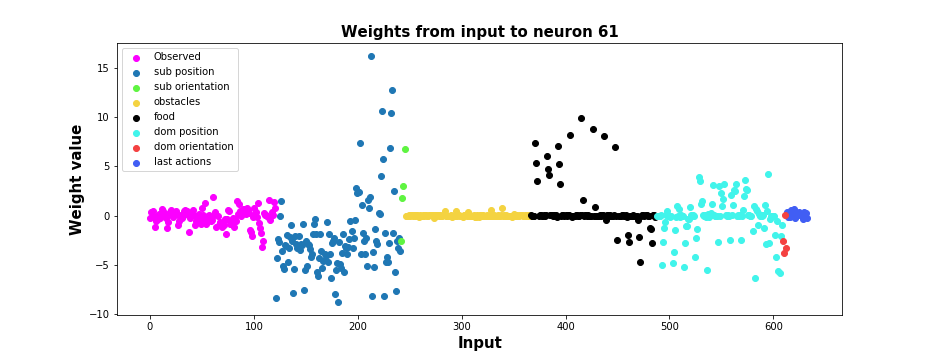
\includegraphics[scale=0.5,trim={3.5cm 0cm 2cm 0.5cm},clip]{figures/PN_61.png}
\caption{Each color represents one group of input e.g (observed area, \(A_{sub}\) position, food position etc..) as explained in section \ref{network.input}. The higher the value, the more weight is assigned to that specific input. Due the high weight assigned to this neuron and the high weights for different food positions in Food map we believe a biological interpretation of neuron 61 might be the agent's desire for food.}
\label{fig.PN_61}
\end{figure}
\begin{figure}[H]
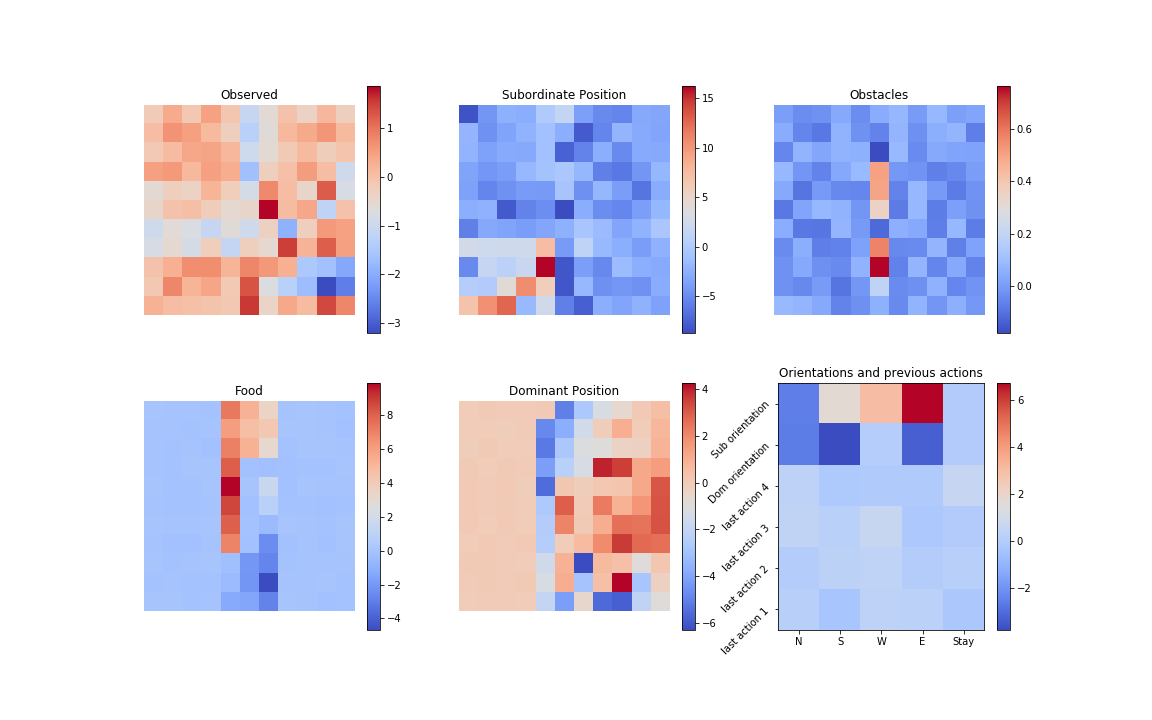
\includegraphics[scale=0.5,trim={5cm 2cm 4cm 3cm},clip]{figures/SN_61.png}
\caption{The weights between the input as explained in section (\ref{network.input}) and neuron 61 in the hidden layer which holds the highest positive weight to the state value node. From this neuron we can see at which location our agent favors each element to be in. We can notice in Food map, that the more food gets closer to the dominant the less favorable the situation is, because it means less probably to get to it and more chance to get punished next to it. This neuron represents the desire for food. From dominant position map we can notice that this neuron gave high values for situations where the dominant is on the other side of the obstacle.}
\label{fig.SN_61}
\end{figure}
\begin{figure}[H]
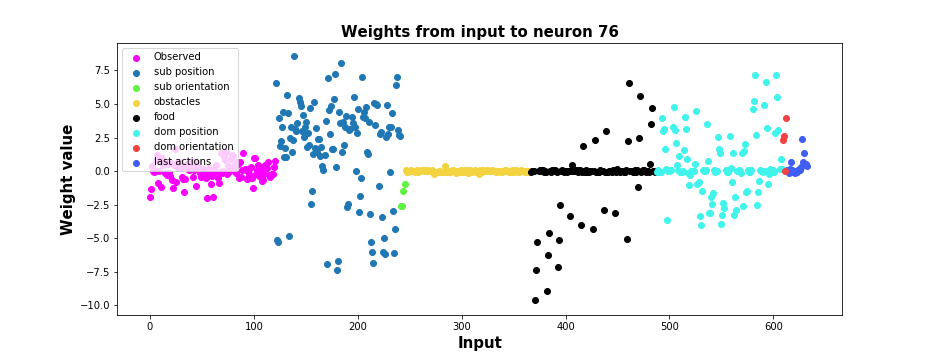
\includegraphics[scale=0.5,trim={3.5cm 0cm 2cm 0.5cm},clip]{figures/PN_76.png}
\caption{Each color represents one group of input e.g (observed area, \(A_{sub}\) position, food position etc..) as explained in section (\ref{network.input}). The higher the value, the more weight is assigned to that specific input. A biological interpretation of neuron 76 might be the agent's fear from dominant.}
\label{fig.PN_76}
\end{figure}
\begin{figure}[H]
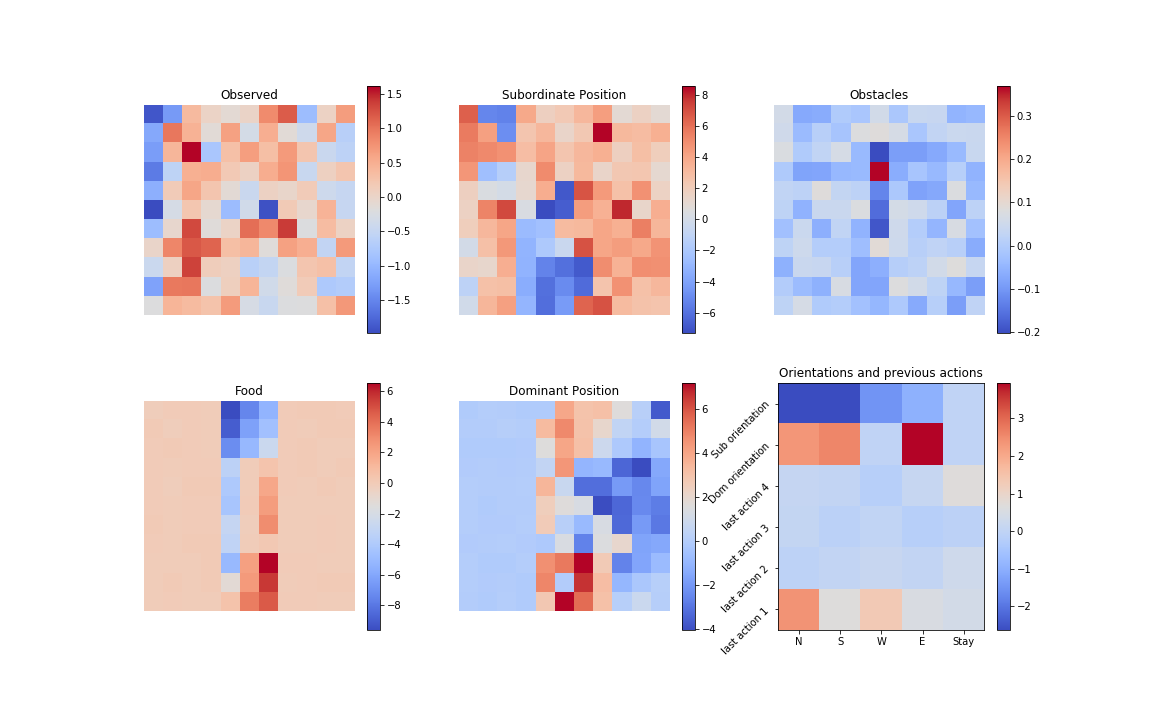
\includegraphics[scale=0.5,trim={5cm 2cm 4cm 3cm},clip]{figures/SN_76.png}
\caption{The weights between the input as explained in section (\ref{network.input}) and neuron 76 in the hidden layer which hold the highest negative weight to the state value node in the next layer. From this neuron we can see where our agent animus each element. We can notice in Food map, that the more food get close to dominant the more  animusable it is. Because it means less probability to get it and more to get punished next to it by dominant. This neuron represents the fear of the dominant. From dominant position map we can notice that this neuron gave high values when the dominant is around the obstacle. Which means more probable negative reward for subordinate.}
\label{fig.SN_76}
\end{figure}
We recorded the hidden nodes values over those 10 cases with variations. Afterward we applied T-SNE to draw the points in 2d. In Figure (\ref{fig.EAB}) we can see the expected and actual behavior of \(A_{sub}\) where we can notice: 1) most of the variation for each test cases tend to be close to each other eg (8,108,208,308,408) which mean the network represent close states close as well. 2) We can notice two separable groups that define when to go or avoid the food.

\begin{figure}[H]
\centering
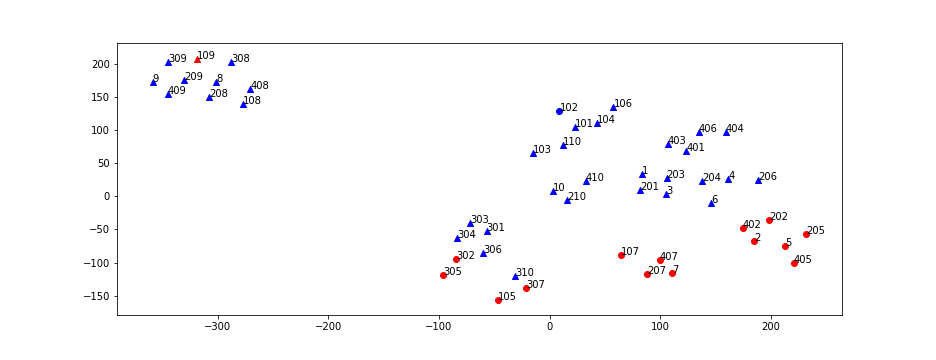
\includegraphics[scale=0.5,,trim={3.5cm , 1.5cm , 0cm , 0cm},clip]{figures/EAB.png}
\caption{T-SNE of the activations over initial states for all 40 test cases (10 test case * 4 variation each). Triangle represent test cases where \(A_{sub}\) is  expected to go toward food, while circles not. Blue represent test cases where \(A_{sub}\) went  to food, while red did not.}
\label{fig.EAB}
\end{figure}

\section{Discussion}
In this paper we showed 10 test cases that require perspective taking to be accomplished. Those test cases and their variations were solved by an artificial neural network trained with RL. The behavior of the agent showed evidence for basic perspective taking skills. By changing only the position of the dominant while keeping the positions of the subordinate, the food and the obstacle the same, we observed that the subordinate either went for the food or not depending on the position of the dominant as shown in Figures \ref{fig.tc.4},\ref{fig.tc.5}. Even when the dominant was in the field of view of the subordinate, the subordinate went for the food if the dominant could not see the food (test case 4, Figure (\ref{fig.tc.4}).  

We also presented a detailed analysis of the weights of the hidden layer and the activation over all the test cases with T-SNE. All T-SNE figures concluded to two clusters which make us believe that the network could be simplified even more by using less neurons in the hidden layer. 

In the present work with relatively simple deep RL agents we observed that the subordinate agent can learn to take into account the behavior of the dominant agent through trial-and-error over a long training period. This is in stark contrast to chimpanzees who master the particular task in the first trial  (Hare et al 2000; 2001). However, it is important to note that the chimpanzees had learned about social hierarchies and about the behavior of other chimpanzees in their daily life over many years. Hence, the fact that in the present work the subordinate agents learned to take into account the behavior of the dominant agent demonstrates that at least part of perspective taking skills can indeed be learned through reinforcement learning. 

We are not claiming that RL would capture all aspects of perspective taking. We simply feel that by understanding the capabilities and limitations of RL agents in acquiring perspective taking we will better understand the computational demands of perspective taking and more generally, of mindreading. In short, RL will help us to better understand perspective taking just as deep neural networks have led to a better understanding of biological vision (Aru \& Vicente, submitted).

In particular the current results show that it is not needed to have a specific Theory of Mind module for agents to show perspective taking behavior: aspects of perspective taking can emerge through relatively simple RL algorithms. Through training these algorithms can learn to take into account subtle cues about the relationships between the other agents and the environmental cues like the position of food and obstacles. In many cases it might be that the position of the elements and orientation is sufficient for the agent to show behavior akin to perspective taking without any need for taking into account what the dominant can or can not see. On one hand it might seem that by studying such simple systems and environments we are missing the gist of human-like perspective taking. But, on the other hand, we would argue that we also need to understand these simpler cue-response contingencies underlying perspective taking. It is important to notice that perspective taking, like any other cognitive ability, has multiple facets and for the scientific understanding such abilities it is necessary to study all of these facets \cite{apperly2011mindreaders}. Here we studied the simplest possible case where agents consisting of relatively simple neural networks learned with the help of reinforcement learning. In our future research we will test other architectures. One straightforward way for improving the present algorithm is to add external memory to the network to make it more similar to the brain. Another way is to incorporate a bias for learning about the other agent: while currently obstacles, food and the other agent were all equal for learning, we know that humans preferentially process signals coming from other humans (i.e. compared to pieces of furniture, falling leaves or sparrows). Endowing the agents with a bias to preferentially process inputs coming from the other agent could be an important step toward building AI agents with more complex mindreading skills (Aru \& Vicente, submitted).

In the end here lies the real advantage of AI research for understanding the brain: in artificial systems one can step-by-step make algorithms more complex and add different algorithms, while monitoring the performance at a particular task. In this fashion, part by part, algorithm by algorithm, it is easier to understand the emergence of complex cognitive functions underlying our intelligence.
\bibliographystyle{plain}
\bibliography{references}
\appendix
\section{Test cases}\label{test.cases}
% the \\ insures the section title is centered below the phrase: AppendixA
Backup test case with subordinate in different position.
\begin{figure}
    \centering
    \subfloat[]{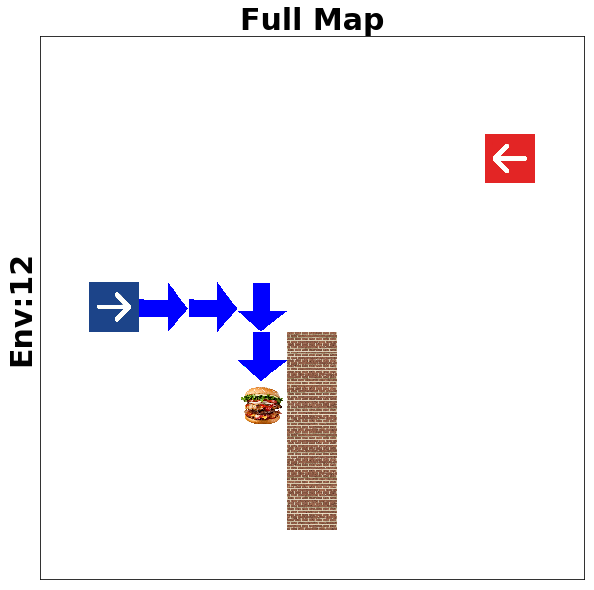
\includegraphics[scale=0.20]{figures/ENV:12_FM.png}}
    \subfloat[]{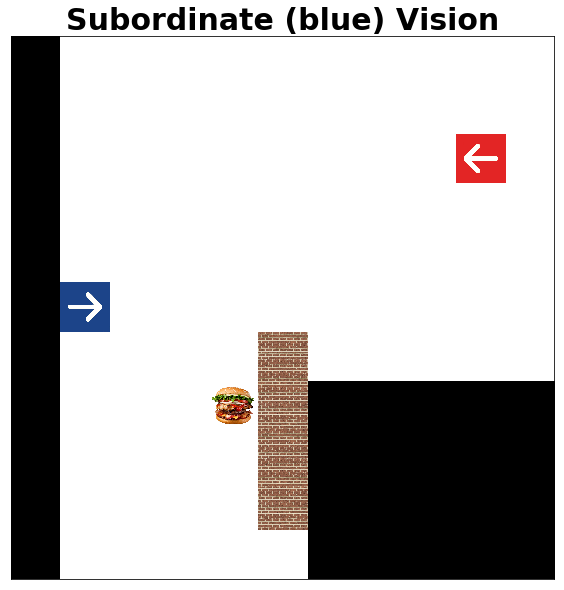
\includegraphics[scale=0.20]{figures/ENV:12_AI.png}}
    \subfloat[]{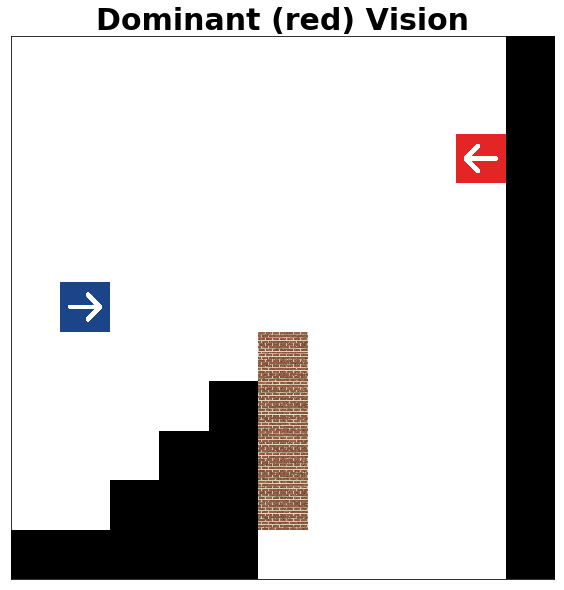
\includegraphics[scale=0.20]{figures/ENV:12_DM.png}}
    \caption{\textbf {Test  case 12:} \(A_{sub}\) can see the food and \(A_{dom}\) where the last can not see the food. \(A_{sub}\) go to food with the arrows trajectory.}
    \label{fig.tc.12}
\end{figure}
\section{Title of Appendix B}
% the \\ insures the section title is centered below the phrase: Appendix B

Text of Appendix B is Here
\end{document}
